% Options for packages loaded elsewhere
\PassOptionsToPackage{unicode}{hyperref}
\PassOptionsToPackage{hyphens}{url}
%
\documentclass[
]{article}
\usepackage{amsmath,amssymb}
\usepackage{lmodern}
\usepackage{iftex}
\ifPDFTeX
  \usepackage[T1]{fontenc}
  \usepackage[utf8]{inputenc}
  \usepackage{textcomp} % provide euro and other symbols
\else % if luatex or xetex
  \usepackage{unicode-math}
  \defaultfontfeatures{Scale=MatchLowercase}
  \defaultfontfeatures[\rmfamily]{Ligatures=TeX,Scale=1}
\fi
% Use upquote if available, for straight quotes in verbatim environments
\IfFileExists{upquote.sty}{\usepackage{upquote}}{}
\IfFileExists{microtype.sty}{% use microtype if available
  \usepackage[]{microtype}
  \UseMicrotypeSet[protrusion]{basicmath} % disable protrusion for tt fonts
}{}
\makeatletter
\@ifundefined{KOMAClassName}{% if non-KOMA class
  \IfFileExists{parskip.sty}{%
    \usepackage{parskip}
  }{% else
    \setlength{\parindent}{0pt}
    \setlength{\parskip}{6pt plus 2pt minus 1pt}}
}{% if KOMA class
  \KOMAoptions{parskip=half}}
\makeatother
\usepackage{xcolor}
\IfFileExists{xurl.sty}{\usepackage{xurl}}{} % add URL line breaks if available
\IfFileExists{bookmark.sty}{\usepackage{bookmark}}{\usepackage{hyperref}}
\hypersetup{
  pdftitle={Statistik und Qualität - Ausarbeitung der ersten Übung},
  pdfauthor={Stefan Dünser},
  hidelinks,
  pdfcreator={LaTeX via pandoc}}
\urlstyle{same} % disable monospaced font for URLs
\usepackage[margin=1in]{geometry}
\usepackage{color}
\usepackage{fancyvrb}
\newcommand{\VerbBar}{|}
\newcommand{\VERB}{\Verb[commandchars=\\\{\}]}
\DefineVerbatimEnvironment{Highlighting}{Verbatim}{commandchars=\\\{\}}
% Add ',fontsize=\small' for more characters per line
\usepackage{framed}
\definecolor{shadecolor}{RGB}{248,248,248}
\newenvironment{Shaded}{\begin{snugshade}}{\end{snugshade}}
\newcommand{\AlertTok}[1]{\textcolor[rgb]{0.94,0.16,0.16}{#1}}
\newcommand{\AnnotationTok}[1]{\textcolor[rgb]{0.56,0.35,0.01}{\textbf{\textit{#1}}}}
\newcommand{\AttributeTok}[1]{\textcolor[rgb]{0.77,0.63,0.00}{#1}}
\newcommand{\BaseNTok}[1]{\textcolor[rgb]{0.00,0.00,0.81}{#1}}
\newcommand{\BuiltInTok}[1]{#1}
\newcommand{\CharTok}[1]{\textcolor[rgb]{0.31,0.60,0.02}{#1}}
\newcommand{\CommentTok}[1]{\textcolor[rgb]{0.56,0.35,0.01}{\textit{#1}}}
\newcommand{\CommentVarTok}[1]{\textcolor[rgb]{0.56,0.35,0.01}{\textbf{\textit{#1}}}}
\newcommand{\ConstantTok}[1]{\textcolor[rgb]{0.00,0.00,0.00}{#1}}
\newcommand{\ControlFlowTok}[1]{\textcolor[rgb]{0.13,0.29,0.53}{\textbf{#1}}}
\newcommand{\DataTypeTok}[1]{\textcolor[rgb]{0.13,0.29,0.53}{#1}}
\newcommand{\DecValTok}[1]{\textcolor[rgb]{0.00,0.00,0.81}{#1}}
\newcommand{\DocumentationTok}[1]{\textcolor[rgb]{0.56,0.35,0.01}{\textbf{\textit{#1}}}}
\newcommand{\ErrorTok}[1]{\textcolor[rgb]{0.64,0.00,0.00}{\textbf{#1}}}
\newcommand{\ExtensionTok}[1]{#1}
\newcommand{\FloatTok}[1]{\textcolor[rgb]{0.00,0.00,0.81}{#1}}
\newcommand{\FunctionTok}[1]{\textcolor[rgb]{0.00,0.00,0.00}{#1}}
\newcommand{\ImportTok}[1]{#1}
\newcommand{\InformationTok}[1]{\textcolor[rgb]{0.56,0.35,0.01}{\textbf{\textit{#1}}}}
\newcommand{\KeywordTok}[1]{\textcolor[rgb]{0.13,0.29,0.53}{\textbf{#1}}}
\newcommand{\NormalTok}[1]{#1}
\newcommand{\OperatorTok}[1]{\textcolor[rgb]{0.81,0.36,0.00}{\textbf{#1}}}
\newcommand{\OtherTok}[1]{\textcolor[rgb]{0.56,0.35,0.01}{#1}}
\newcommand{\PreprocessorTok}[1]{\textcolor[rgb]{0.56,0.35,0.01}{\textit{#1}}}
\newcommand{\RegionMarkerTok}[1]{#1}
\newcommand{\SpecialCharTok}[1]{\textcolor[rgb]{0.00,0.00,0.00}{#1}}
\newcommand{\SpecialStringTok}[1]{\textcolor[rgb]{0.31,0.60,0.02}{#1}}
\newcommand{\StringTok}[1]{\textcolor[rgb]{0.31,0.60,0.02}{#1}}
\newcommand{\VariableTok}[1]{\textcolor[rgb]{0.00,0.00,0.00}{#1}}
\newcommand{\VerbatimStringTok}[1]{\textcolor[rgb]{0.31,0.60,0.02}{#1}}
\newcommand{\WarningTok}[1]{\textcolor[rgb]{0.56,0.35,0.01}{\textbf{\textit{#1}}}}
\usepackage{graphicx}
\makeatletter
\def\maxwidth{\ifdim\Gin@nat@width>\linewidth\linewidth\else\Gin@nat@width\fi}
\def\maxheight{\ifdim\Gin@nat@height>\textheight\textheight\else\Gin@nat@height\fi}
\makeatother
% Scale images if necessary, so that they will not overflow the page
% margins by default, and it is still possible to overwrite the defaults
% using explicit options in \includegraphics[width, height, ...]{}
\setkeys{Gin}{width=\maxwidth,height=\maxheight,keepaspectratio}
% Set default figure placement to htbp
\makeatletter
\def\fps@figure{htbp}
\makeatother
\setlength{\emergencystretch}{3em} % prevent overfull lines
\providecommand{\tightlist}{%
  \setlength{\itemsep}{0pt}\setlength{\parskip}{0pt}}
\setcounter{secnumdepth}{-\maxdimen} % remove section numbering
\ifLuaTeX
  \usepackage{selnolig}  % disable illegal ligatures
\fi

\title{Statistik und Qualität - Ausarbeitung der ersten Übung}
\author{Stefan Dünser}
\date{}

\begin{document}
\maketitle

\hypertarget{a-technische-fertigkeiten}{%
\section{\texorpdfstring{A) TECHNISCHE FERTIGKEITEN\\
}{A) TECHNISCHE FERTIGKEITEN }}\label{a-technische-fertigkeiten}}

\hypertarget{a-1-handelt-es-sich-bei-den-vorliegenden-statistischen-gesamtheiten-um-bestands--oder-bewegungsgruxf6uxdfen}{%
\subsubsection{A-1) Handelt es sich bei den vorliegenden statistischen
Gesamtheiten um Bestands- oder
Bewegungsgrößen?}\label{a-1-handelt-es-sich-bei-den-vorliegenden-statistischen-gesamtheiten-um-bestands--oder-bewegungsgruxf6uxdfen}}

\begin{itemize}
\tightlist
\item
  \textbf{a) Studierende an einer Hochschule.}

  \begin{itemize}
  \tightlist
  \item
    Bestandsgröße
  \end{itemize}
\item
  \textbf{b) Hochzeiten am Standesamt einer Gemeinde.}

  \begin{itemize}
  \tightlist
  \item
    Bewegungsgröße
  \end{itemize}
\item
  \textbf{c) Bei der Behörde gemeldete Personenkraftwagen.}

  \begin{itemize}
  \tightlist
  \item
    Bestandsgröße
  \end{itemize}
\item
  \textbf{d) Maschinenausfälle in einer Werkstatt.}

  \begin{itemize}
  \tightlist
  \item
    Bewegungsgröße
  \end{itemize}
\item
  \textbf{e) Wartende Kunden vor einem Abfertigungsschalter.}

  \begin{itemize}
  \tightlist
  \item
    Bestandsgröße
  \end{itemize}
\end{itemize}

\hypertarget{a-2-im-servicecenter-eines-unternehmens-werden-uxfcber-einen-zeitraum-eines-tages-die-eingehenden-anrufe-aufgezeichnet.-gezuxe4hlt-wird-die-anzahl-der-pro-10-minuten-zeitintervall-eingehenden-anrufe.-fuxfcr-40-derartige-zeitintervalle-erhuxe4lt-man-folgende-ergebnisse}{%
\subsubsection{A-2) Im Servicecenter eines Unternehmens werden über
einen Zeitraum eines Tages die eingehenden Anrufe aufgezeichnet. Gezählt
wird die Anzahl der pro 10-Minuten-Zeitintervall eingehenden Anrufe. Für
40 derartige Zeitintervalle erhält man folgende
Ergebnisse:}\label{a-2-im-servicecenter-eines-unternehmens-werden-uxfcber-einen-zeitraum-eines-tages-die-eingehenden-anrufe-aufgezeichnet.-gezuxe4hlt-wird-die-anzahl-der-pro-10-minuten-zeitintervall-eingehenden-anrufe.-fuxfcr-40-derartige-zeitintervalle-erhuxe4lt-man-folgende-ergebnisse}}

\begin{Shaded}
\begin{Highlighting}[]
\NormalTok{Liste.vec }\OtherTok{\textless{}{-}} \FunctionTok{c}\NormalTok{(}\DecValTok{0}\NormalTok{, }\DecValTok{0}\NormalTok{, }\DecValTok{1}\NormalTok{, }\DecValTok{3}\NormalTok{, }\DecValTok{4}\NormalTok{, }\DecValTok{1}\NormalTok{, }\DecValTok{2}\NormalTok{, }\DecValTok{2}\NormalTok{, }\DecValTok{1}\NormalTok{, }\DecValTok{1}\NormalTok{, }\DecValTok{1}\NormalTok{, }\DecValTok{2}\NormalTok{, }\DecValTok{3}\NormalTok{, }\DecValTok{0}\NormalTok{, }\DecValTok{2}\NormalTok{, }\DecValTok{0}\NormalTok{, }\DecValTok{1}\NormalTok{, }\DecValTok{3}\NormalTok{, }\DecValTok{1}\NormalTok{, }\DecValTok{2}\NormalTok{, }\DecValTok{2}\NormalTok{, }\DecValTok{0}\NormalTok{, }\DecValTok{1}\NormalTok{, }\DecValTok{1}\NormalTok{, }\DecValTok{6}\NormalTok{, }\DecValTok{1}\NormalTok{, }\DecValTok{0}\NormalTok{, }\DecValTok{2}\NormalTok{, }\DecValTok{3}\NormalTok{, }\DecValTok{1}\NormalTok{, }\DecValTok{1}\NormalTok{, }\DecValTok{4}\NormalTok{, }\DecValTok{2}\NormalTok{, }\DecValTok{3}\NormalTok{, }\DecValTok{2}\NormalTok{, }\DecValTok{0}\NormalTok{, }\DecValTok{3}\NormalTok{, }\DecValTok{0}\NormalTok{, }\DecValTok{1}\NormalTok{, }\DecValTok{2}\NormalTok{)}
\NormalTok{Liste.vec}
\end{Highlighting}
\end{Shaded}

\begin{verbatim}
##  [1] 0 0 1 3 4 1 2 2 1 1 1 2 3 0 2 0 1 3 1 2 2 0 1 1 6 1 0 2 3 1 1 4 2 3 2 0 3 0
## [39] 1 2
\end{verbatim}

\hypertarget{a-was-stellt-bei-dieser-fragestellung-die-statistische-grundgesamtheit-dar-was-sind-die-beobachteten-merkmale-der-statistischen-einheiten-und-wie-sind-sie-skaliert}{%
\subparagraph{\texorpdfstring{\textbf{a) Was stellt bei dieser
Fragestellung die statistische Grundgesamtheit dar? Was sind die
beobachteten Merkmale der statistischen Einheiten und wie sind sie
skaliert?}}{a) Was stellt bei dieser Fragestellung die statistische Grundgesamtheit dar? Was sind die beobachteten Merkmale der statistischen Einheiten und wie sind sie skaliert?}}\label{a-was-stellt-bei-dieser-fragestellung-die-statistische-grundgesamtheit-dar-was-sind-die-beobachteten-merkmale-der-statistischen-einheiten-und-wie-sind-sie-skaliert}}

\begin{itemize}
\tightlist
\item
  Grundgesamtheit

  \begin{itemize}
  \tightlist
  \item
    Die Grundgesamtheit setzt sich auch sen statistischen Einheiten
    zusammen. Die Grundgesamtheit sind die Anzahl der
    10-Minuten-Zeitintervalle - (40).
  \end{itemize}
\item
  Merkmale

  \begin{itemize}
  \tightlist
  \item
    Anzahl der 10-Minuten-Zeitintervalle (40)
  \item
    Anzahl der Anrufe über alle Zeitintervalle (65)
  \end{itemize}
\item
  Skalierung

  \begin{itemize}
  \tightlist
  \item
    Metrische Skalierung (Kardinalskala), die verhältnisskaliert ist
  \end{itemize}
\end{itemize}

\hypertarget{b-ermittle-die-absolute-und-relative-huxe4ufigkeitstabelle-der-eingehenden-anrufe-und-stelle-die-huxe4ufigkeitsverteilung-und-summenhuxe4ufigkeit-grafisch-dar.}{%
\subparagraph{\texorpdfstring{\textbf{b) Ermittle die absolute und
relative Häufigkeitstabelle der eingehenden Anrufe und stelle die
Häufigkeitsverteilung und Summenhäufigkeit grafisch
dar.}}{b) Ermittle die absolute und relative Häufigkeitstabelle der eingehenden Anrufe und stelle die Häufigkeitsverteilung und Summenhäufigkeit grafisch dar.}}\label{b-ermittle-die-absolute-und-relative-huxe4ufigkeitstabelle-der-eingehenden-anrufe-und-stelle-die-huxe4ufigkeitsverteilung-und-summenhuxe4ufigkeit-grafisch-dar.}}

\hypertarget{absolute-huxe4ufigkeit}{%
\subparagraph{\texorpdfstring{\textbf{Absolute
Häufigkeit:}}{Absolute Häufigkeit:}}\label{absolute-huxe4ufigkeit}}

\begin{Shaded}
\begin{Highlighting}[]
\FunctionTok{table}\NormalTok{(Liste.vec)}
\end{Highlighting}
\end{Shaded}

\begin{verbatim}
## Liste.vec
##  0  1  2  3  4  6 
##  8 13 10  6  2  1
\end{verbatim}

\begin{Shaded}
\begin{Highlighting}[]
\FunctionTok{barplot}\NormalTok{(}\FunctionTok{table}\NormalTok{(}\FunctionTok{factor}\NormalTok{(Liste.vec,}\AttributeTok{levels=}\FunctionTok{c}\NormalTok{(}\DecValTok{0}\NormalTok{,}\DecValTok{1}\NormalTok{,}\DecValTok{2}\NormalTok{,}\DecValTok{3}\NormalTok{,}\DecValTok{4}\NormalTok{,}\DecValTok{5}\NormalTok{,}\DecValTok{6}\NormalTok{))), }\AttributeTok{ylim =} \FunctionTok{c}\NormalTok{(}\DecValTok{0}\NormalTok{,}\DecValTok{15}\NormalTok{), }\AttributeTok{xlab =} \StringTok{"Anzahl der Anrufe innerhalb eines 10{-}Minuten\_Zeitintervalls"}\NormalTok{, }\AttributeTok{ylab =} \StringTok{"Absolute Häufigkeit"}\NormalTok{, }\AttributeTok{main =} \StringTok{"Absolute Häufigkeitsverteilung"}\NormalTok{, }\AttributeTok{col.main =} \StringTok{"darkblue"}\NormalTok{, }\AttributeTok{col =} \StringTok{"blue"}\NormalTok{)}
\end{Highlighting}
\end{Shaded}

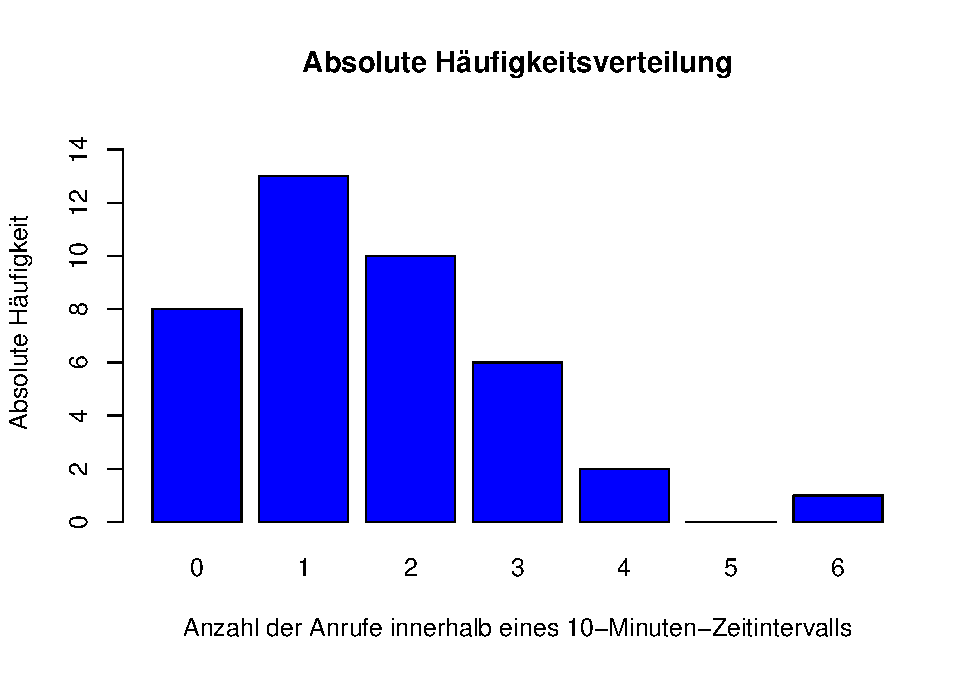
\includegraphics{Uebung1_StefanDuenser_files/figure-latex/unnamed-chunk-3-1.pdf}

\hypertarget{relative-huxe4ufigkeit}{%
\subparagraph{\texorpdfstring{\textbf{Relative
Häufigkeit:}}{Relative Häufigkeit:}}\label{relative-huxe4ufigkeit}}

\begin{Shaded}
\begin{Highlighting}[]
\FunctionTok{table}\NormalTok{(Liste.vec)}\SpecialCharTok{/}\FunctionTok{length}\NormalTok{(Liste.vec)}
\end{Highlighting}
\end{Shaded}

\begin{verbatim}
## Liste.vec
##     0     1     2     3     4     6 
## 0.200 0.325 0.250 0.150 0.050 0.025
\end{verbatim}

\begin{Shaded}
\begin{Highlighting}[]
\FunctionTok{barplot}\NormalTok{(}\FunctionTok{table}\NormalTok{(}\FunctionTok{factor}\NormalTok{(Liste.vec,}\AttributeTok{levels=}\FunctionTok{c}\NormalTok{(}\DecValTok{0}\NormalTok{,}\DecValTok{1}\NormalTok{,}\DecValTok{2}\NormalTok{,}\DecValTok{3}\NormalTok{,}\DecValTok{4}\NormalTok{,}\DecValTok{5}\NormalTok{,}\DecValTok{6}\NormalTok{)))}\SpecialCharTok{/}\FunctionTok{sum}\NormalTok{(}\FunctionTok{table}\NormalTok{(Liste.vec)), }\AttributeTok{ylim =} \FunctionTok{c}\NormalTok{(}\DecValTok{0}\NormalTok{,}\FloatTok{0.4}\NormalTok{), }\AttributeTok{xlab =} \StringTok{"Anzahl der Anrufe innerhalb eines 10 min Zeitintervalls"}\NormalTok{,}\AttributeTok{ylab =} \StringTok{"relative Häufigkeit"}\NormalTok{, }\AttributeTok{main =} \StringTok{"Relative Häufigkeitsverteilung"}\NormalTok{, }\AttributeTok{col.main =} \StringTok{"darkblue"}\NormalTok{, }\AttributeTok{col =} \StringTok{"blue"}\NormalTok{)}
\end{Highlighting}
\end{Shaded}

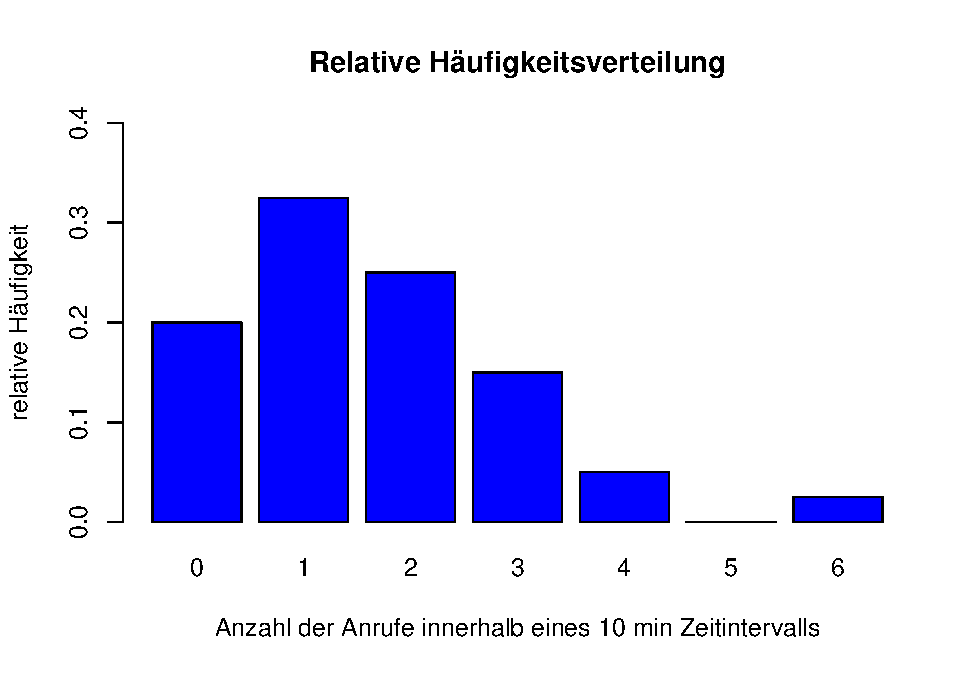
\includegraphics{Uebung1_StefanDuenser_files/figure-latex/unnamed-chunk-5-1.pdf}
\#\#\#\#\# \textbf{Summenhäufigkeit}

\begin{Shaded}
\begin{Highlighting}[]
\FunctionTok{cumsum}\NormalTok{(}\FunctionTok{table}\NormalTok{(Liste.vec))}
\end{Highlighting}
\end{Shaded}

\begin{verbatim}
##  0  1  2  3  4  6 
##  8 21 31 37 39 40
\end{verbatim}

\begin{Shaded}
\begin{Highlighting}[]
\FunctionTok{barplot}\NormalTok{(}\FunctionTok{cumsum}\NormalTok{(}\FunctionTok{table}\NormalTok{(}\FunctionTok{factor}\NormalTok{(Liste.vec,}\AttributeTok{levels =} \FunctionTok{c}\NormalTok{(}\DecValTok{0}\NormalTok{,}\DecValTok{1}\NormalTok{,}\DecValTok{2}\NormalTok{,}\DecValTok{3}\NormalTok{,}\DecValTok{4}\NormalTok{,}\DecValTok{5}\NormalTok{,}\DecValTok{6}\NormalTok{))))}\SpecialCharTok{/}\FunctionTok{sum}\NormalTok{(}\FunctionTok{table}\NormalTok{(Liste.vec)), }\AttributeTok{xlab =} \StringTok{"Anzahl der Anrufe innerhalb des Intervalls"}\NormalTok{, }\AttributeTok{ylab =} \StringTok{"Relative Summenhäufigkeit"}\NormalTok{, }\AttributeTok{main =} \StringTok{"Summenhäufigkeit"}\NormalTok{, }\AttributeTok{col.main =} \StringTok{"darkblue"}\NormalTok{, }\AttributeTok{col =} \StringTok{"blue"}\NormalTok{)}
\FunctionTok{abline}\NormalTok{(}\FloatTok{0.25}\NormalTok{, }\DecValTok{0}\NormalTok{, }\AttributeTok{lty =} \StringTok{"dashed"}\NormalTok{)}
\FunctionTok{abline}\NormalTok{(}\FloatTok{0.5}\NormalTok{, }\DecValTok{0}\NormalTok{, }\AttributeTok{lty =} \StringTok{"dashed"}\NormalTok{, }\AttributeTok{col =} \StringTok{"red"}\NormalTok{)}
\FunctionTok{abline}\NormalTok{(}\FloatTok{0.75}\NormalTok{, }\DecValTok{0}\NormalTok{, }\AttributeTok{lty =} \StringTok{"dashed"}\NormalTok{)}
\end{Highlighting}
\end{Shaded}

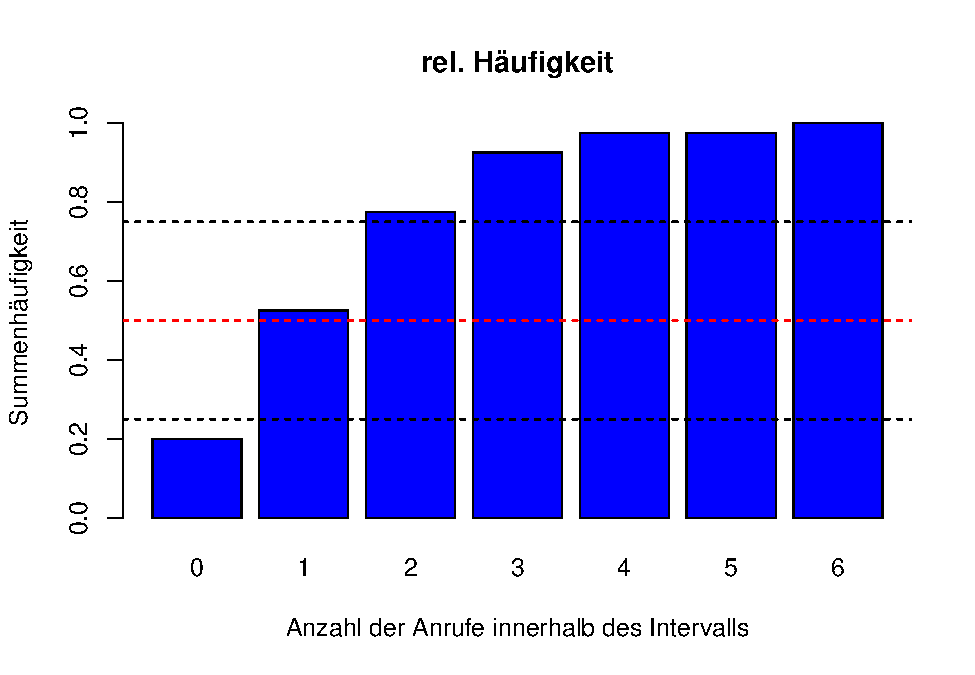
\includegraphics{Uebung1_StefanDuenser_files/figure-latex/unnamed-chunk-7-1.pdf}

\hypertarget{c-schuxe4tze-das-arithmetische-mittel-aus-der-grafischen-darstellung-fuxfcr-die-huxe4ufigkeit-und-den-median-aus-der-grafischen-darstellung-fuxfcr-die-summenhuxe4ufigkeit.}{%
\subparagraph{\texorpdfstring{\textbf{c) Schätze das arithmetische
Mittel aus der grafischen Darstellung für die Häufigkeit und den Median
aus der grafischen Darstellung für die
Summenhäufigkeit.}}{c) Schätze das arithmetische Mittel aus der grafischen Darstellung für die Häufigkeit und den Median aus der grafischen Darstellung für die Summenhäufigkeit.}}\label{c-schuxe4tze-das-arithmetische-mittel-aus-der-grafischen-darstellung-fuxfcr-die-huxe4ufigkeit-und-den-median-aus-der-grafischen-darstellung-fuxfcr-die-summenhuxe4ufigkeit.}}

\textbf{Arithmetisches Mittel:} Das arithmestische Mittel kann als
Schwerpunkt der Häufigkeitsverteilung angesehen werden. In diesem Fall
beträgt das arithmetische Mittel nach Abschätzung rund 1,5, da somit
links und rechts der x-Achse in etwa gleich viele Werte sind.
\textbf{Median:} Der Median wird über die y-Achse ermittelt. Der Median
befindet sich dann auf der x-Achse an dem Punkt, an dem 50\% des y-Werts
erreicht sind. In diesem Fall ist der Median bei 1.

\hypertarget{d-berechne-die-muxf6glichen-lageparameter-zentralmauxdfe-und-streumauxdfe}{%
\subparagraph{\texorpdfstring{\textbf{d) Berechne die möglichen
Lageparameter (Zentralmaße und
Streumaße)}}{d) Berechne die möglichen Lageparameter (Zentralmaße und Streumaße)}}\label{d-berechne-die-muxf6glichen-lageparameter-zentralmauxdfe-und-streumauxdfe}}

\textbf{Zentralmaße:}\\
\textbf{\emph{Modus}}

\begin{Shaded}
\begin{Highlighting}[]
\NormalTok{getmode }\OtherTok{\textless{}{-}} \ControlFlowTok{function}\NormalTok{(Liste.vec) \{}
\NormalTok{   uniqv }\OtherTok{\textless{}{-}} \FunctionTok{unique}\NormalTok{(Liste.vec)}
\NormalTok{   uniqv[}\FunctionTok{which.max}\NormalTok{(}\FunctionTok{tabulate}\NormalTok{(}\FunctionTok{match}\NormalTok{(Liste.vec, uniqv)))]}
\NormalTok{\}}
\NormalTok{mode }\OtherTok{\textless{}{-}} \FunctionTok{getmode}\NormalTok{(Liste.vec)}
\NormalTok{mode}
\end{Highlighting}
\end{Shaded}

\begin{verbatim}
## [1] 1
\end{verbatim}

\textbf{Median}

\begin{Shaded}
\begin{Highlighting}[]
\FunctionTok{median}\NormalTok{(Liste.vec)}
\end{Highlighting}
\end{Shaded}

\begin{verbatim}
## [1] 1
\end{verbatim}

\textbf{Arithmetisches Mittel}

\begin{Shaded}
\begin{Highlighting}[]
\FunctionTok{mean}\NormalTok{(Liste.vec)}
\end{Highlighting}
\end{Shaded}

\begin{verbatim}
## [1] 1.625
\end{verbatim}

\hfill\break
\textbf{\emph{Streumaße:}} Minimum

\begin{Shaded}
\begin{Highlighting}[]
\NormalTok{Minimum }\OtherTok{\textless{}{-}} \FunctionTok{min}\NormalTok{(Liste.vec)}
\NormalTok{Minimum}
\end{Highlighting}
\end{Shaded}

\begin{verbatim}
## [1] 0
\end{verbatim}

\textbf{Maximum}

\begin{Shaded}
\begin{Highlighting}[]
\NormalTok{Maximum }\OtherTok{\textless{}{-}} \FunctionTok{max}\NormalTok{(Liste.vec)}
\NormalTok{Maximum}
\end{Highlighting}
\end{Shaded}

\begin{verbatim}
## [1] 6
\end{verbatim}

\textbf{Spannweite}

\begin{Shaded}
\begin{Highlighting}[]
\NormalTok{Spannweite }\OtherTok{\textless{}{-}} \FunctionTok{range}\NormalTok{(Liste.vec)}
\NormalTok{Spannweite}
\end{Highlighting}
\end{Shaded}

\begin{verbatim}
## [1] 0 6
\end{verbatim}

\textbf{Quantile}

\begin{Shaded}
\begin{Highlighting}[]
\FunctionTok{quantile}\NormalTok{(Liste.vec)}
\end{Highlighting}
\end{Shaded}

\begin{verbatim}
##   0%  25%  50%  75% 100% 
##    0    1    1    2    6
\end{verbatim}

\textbf{Mittlere absolute Abweichung}

\begin{Shaded}
\begin{Highlighting}[]
\FunctionTok{mean}\NormalTok{(}\FunctionTok{abs}\NormalTok{(Liste.vec}\SpecialCharTok{{-}}\FunctionTok{mean}\NormalTok{(Liste.vec)))}
\end{Highlighting}
\end{Shaded}

\begin{verbatim}
## [1] 1.05625
\end{verbatim}

\textbf{Standardabweichung}

\begin{Shaded}
\begin{Highlighting}[]
\FunctionTok{sd}\NormalTok{(Liste.vec)}
\end{Highlighting}
\end{Shaded}

\begin{verbatim}
## [1] 1.333734
\end{verbatim}

\hypertarget{e-stelle-die-daten-in-einem-boxplot-dar}{%
\subparagraph{\texorpdfstring{\textbf{e) Stelle die Daten in einem
Boxplot
dar}}{e) Stelle die Daten in einem Boxplot dar}}\label{e-stelle-die-daten-in-einem-boxplot-dar}}

\begin{Shaded}
\begin{Highlighting}[]
\FunctionTok{boxplot}\NormalTok{(Liste.vec, }\AttributeTok{col =} \StringTok{"blue"}\NormalTok{)}
\end{Highlighting}
\end{Shaded}

\includegraphics{Uebung1_StefanDuenser_files/figure-latex/unnamed-chunk-17-1.pdf}\\
Besonders Auffällig ist bei diesem Boxplot bzw. den Werten aus der
Liste, dass der Median und das erste Quartil (25\% Quantil)
zusammenfallen. Die Werte 4 Anrufe sowie 6 Anrufe innerhalb eines
10-Minuten\_Zeitintervalls werden hier als Ausreißer aufgefasst und als
Kreis dargestellt.

\hypertarget{a-3-eine-anzahl-von-1000-kleinmotoren-weist-folgende-lebensdauer-auf}{%
\subsubsection{A-3) Eine Anzahl von 1000 Kleinmotoren weist folgende
Lebensdauer
auf:}\label{a-3-eine-anzahl-von-1000-kleinmotoren-weist-folgende-lebensdauer-auf}}

\begin{Shaded}
\begin{Highlighting}[]
\NormalTok{AnzahlMotoren }\OtherTok{\textless{}{-}} \FunctionTok{c}\NormalTok{(}\DecValTok{33}\NormalTok{,}\DecValTok{276}\NormalTok{,}\DecValTok{404}\NormalTok{,}\DecValTok{237}\NormalTok{,}\DecValTok{50}\NormalTok{)}
\NormalTok{Lebensdauer }\OtherTok{\textless{}{-}} \FunctionTok{c}\NormalTok{(}\DecValTok{0}\SpecialCharTok{:}\DecValTok{10}\NormalTok{)}
\end{Highlighting}
\end{Shaded}

\hypertarget{a-stelle-die-huxe4ufigkeitsverteilung-und-summenhuxe4ufigkeit-grafisch-dar.}{%
\subparagraph{\texorpdfstring{\textbf{a) Stelle die
Häufigkeitsverteilung und Summenhäufigkeit grafisch
dar.}}{a) Stelle die Häufigkeitsverteilung und Summenhäufigkeit grafisch dar.}}\label{a-stelle-die-huxe4ufigkeitsverteilung-und-summenhuxe4ufigkeit-grafisch-dar.}}

\hypertarget{b-schuxe4tze-das-arithmetische-mittel-aus-der-grafischen-darstellung-fuxfcr-die-huxe4ufigkeit-und-den-median-aus-der-grafischen-darstellung-fuxfcr-die-summenhuxe4ufigkeit.}{%
\subparagraph{\texorpdfstring{\textbf{b) Schätze das arithmetische
Mittel aus der grafischen Darstellung für die Häufigkeit und den Median
aus der grafischen Darstellung für die
Summenhäufigkeit.}}{b) Schätze das arithmetische Mittel aus der grafischen Darstellung für die Häufigkeit und den Median aus der grafischen Darstellung für die Summenhäufigkeit.}}\label{b-schuxe4tze-das-arithmetische-mittel-aus-der-grafischen-darstellung-fuxfcr-die-huxe4ufigkeit-und-den-median-aus-der-grafischen-darstellung-fuxfcr-die-summenhuxe4ufigkeit.}}

\hypertarget{c-bestimme-der-anteil-der-motoren-mit-uxfcber-6-jahren-lebensdauer.}{%
\subparagraph{\texorpdfstring{\textbf{c) Bestimme der Anteil der Motoren
mit über 6 Jahren
Lebensdauer.}}{c) Bestimme der Anteil der Motoren mit über 6 Jahren Lebensdauer.}}\label{c-bestimme-der-anteil-der-motoren-mit-uxfcber-6-jahren-lebensdauer.}}

\hypertarget{d-berechne-die-muxf6glichen-lageparameter-zentralmauxdfe-und-streumauxdfe.}{%
\subparagraph{\texorpdfstring{\textbf{d) Berechne die möglichen
Lageparameter (Zentralmaße und
Streumaße).}}{d) Berechne die möglichen Lageparameter (Zentralmaße und Streumaße).}}\label{d-berechne-die-muxf6glichen-lageparameter-zentralmauxdfe-und-streumauxdfe.}}

\hypertarget{a-4-ein-technisches-servicecenter-zeichnet-an-100-tagen-die-huxe4ufigkeit-der-einsuxe4tze-auf.-es-ergibt-sich-folgende-tabelle}{%
\subsubsection{A-4) Ein technisches Servicecenter zeichnet an 100 Tagen
die Häufigkeit der Einsätze auf. Es ergibt sich folgende
Tabelle:}\label{a-4-ein-technisches-servicecenter-zeichnet-an-100-tagen-die-huxe4ufigkeit-der-einsuxe4tze-auf.-es-ergibt-sich-folgende-tabelle}}

\begin{Shaded}
\begin{Highlighting}[]
\NormalTok{AnzahlTage }\OtherTok{\textless{}{-}} \FunctionTok{c}\NormalTok{(}\DecValTok{16}\NormalTok{,}\DecValTok{48}\NormalTok{,}\DecValTok{27}\NormalTok{,}\DecValTok{9}\NormalTok{)}
\NormalTok{AnzahlEinsaetze }\OtherTok{\textless{}{-}} \FunctionTok{c}\NormalTok{(}\DecValTok{0}\SpecialCharTok{:}\DecValTok{80}\NormalTok{)}
\end{Highlighting}
\end{Shaded}

\hypertarget{a-stelle-die-huxe4ufigkeitsverteilung-und-summenhuxe4ufigkeit-grafisch-dar.-1}{%
\subparagraph{\texorpdfstring{\textbf{a) Stelle die
Häufigkeitsverteilung und Summenhäufigkeit grafisch
dar.}}{a) Stelle die Häufigkeitsverteilung und Summenhäufigkeit grafisch dar.}}\label{a-stelle-die-huxe4ufigkeitsverteilung-und-summenhuxe4ufigkeit-grafisch-dar.-1}}

\hypertarget{b-schuxe4tze-das-arithmetische-mittel-aus-der-grafischen-darstellung-fuxfcr-die-huxe4ufigkeit-und-den-median-aus-der-grafischen-darstellung-fuxfcr-die-summenhuxe4ufigkeit.-1}{%
\subparagraph{\texorpdfstring{\textbf{b) Schätze das arithmetische
Mittel aus der grafischen Darstellung für die Häufigkeit und den Median
aus der grafischen Darstellung für die
Summenhäufigkeit.}}{b) Schätze das arithmetische Mittel aus der grafischen Darstellung für die Häufigkeit und den Median aus der grafischen Darstellung für die Summenhäufigkeit.}}\label{b-schuxe4tze-das-arithmetische-mittel-aus-der-grafischen-darstellung-fuxfcr-die-huxe4ufigkeit-und-den-median-aus-der-grafischen-darstellung-fuxfcr-die-summenhuxe4ufigkeit.-1}}

\hypertarget{c-bestimme-der-anteil-der-tage-mit-uxfcber-20-einsuxe4tzen.}{%
\subparagraph{\texorpdfstring{\textbf{c) Bestimme der Anteil der Tage
mit über 20
Einsätzen.}}{c) Bestimme der Anteil der Tage mit über 20 Einsätzen.}}\label{c-bestimme-der-anteil-der-tage-mit-uxfcber-20-einsuxe4tzen.}}

\hypertarget{d-berechne-die-muxf6glichen-lageparameter-zentralmauxdfe-und-streumauxdfe.-welcher-aspekt-kuxf6nnte-hier-problematisch-sein-warum}{%
\subparagraph{\texorpdfstring{\textbf{d) Berechne die möglichen
Lageparameter (Zentralmaße und Streumaße). Welcher Aspekt könnte hier
problematisch sein?
Warum?}}{d) Berechne die möglichen Lageparameter (Zentralmaße und Streumaße). Welcher Aspekt könnte hier problematisch sein? Warum?}}\label{d-berechne-die-muxf6glichen-lageparameter-zentralmauxdfe-und-streumauxdfe.-welcher-aspekt-kuxf6nnte-hier-problematisch-sein-warum}}

\hypertarget{b-verstuxe4ndnisfragen}{%
\section{B) VERSTÄNDNISFRAGEN}\label{b-verstuxe4ndnisfragen}}

\hypertarget{b-1-zeige-dass-das-arithmetische-mittel-unter-dem-schwerpunkt-der-huxe4ufigkeitsfunktion-liegt.}{%
\subsubsection{B-1) Zeige, dass das arithmetische Mittel unter dem
Schwerpunkt der Häufigkeitsfunktion
liegt.}\label{b-1-zeige-dass-das-arithmetische-mittel-unter-dem-schwerpunkt-der-huxe4ufigkeitsfunktion-liegt.}}

\hypertarget{b-2-verschiebungssatz-zur-berechnung-der-standardabweichung-das-arithmetische-mittel-ist-gegeben-durch-mu-und-die-varianz-ist-definiert-als-sigm2.-zeige-die-direkte-umformung-dass-daraus-folgt-verschiebungssatz-sigm2}{%
\subsubsection{\texorpdfstring{B-2) Verschiebungssatz zur Berechnung der
Standardabweichung:~Das arithmetische Mittel ist gegeben durch
\(\mu\ =\ \) und die Varianz ist definiert als \(\sigm^2\).~Zeige die
direkte Umformung, dass daraus folgt
(Verschiebungssatz):~\[\sigm^2\ =\ \]}{B-2) Verschiebungssatz zur Berechnung der Standardabweichung:~Das arithmetische Mittel ist gegeben durch \textbackslash mu\textbackslash{} =\textbackslash{}  und die Varianz ist definiert als \textbackslash sigm\^{}2.~Zeige die direkte Umformung, dass daraus folgt (Verschiebungssatz):~\textbackslash sigm\^{}2\textbackslash{} =\textbackslash{} }}\label{b-2-verschiebungssatz-zur-berechnung-der-standardabweichung-das-arithmetische-mittel-ist-gegeben-durch-mu-und-die-varianz-ist-definiert-als-sigm2.-zeige-die-direkte-umformung-dass-daraus-folgt-verschiebungssatz-sigm2}}

\end{document}
